\documentclass[fontsize=11pt,%
twoside,% oneside als Alternative m\"{o}glich
BCOR          = 8mm, % bei Bedarf anzupassen
DIV           = 11,  % kann nach Belieben geändert werden
titlepage     = off,%
index=totoc,%
xcolor        = pdftex,%
dvipsnames,%
bibliography  = totoc,%
bibliography = numbered, % bei Bedarf einschalten
listof        = notnumbered]{scrreprt}

\usepackage[left=3.5cm,right=2cm,top=2.5cm,bottom=2cm]{geometry}
\usepackage[english]{babel}                         %deutsches Sprachpacket
\usepackage[utf8]{inputenc}                         %input utf8
\usepackage[official]{eurosym}                      %Symbolsatz
\usepackage{amsmath}                                %Mathepacket
\usepackage{siunitx}                                %Package für zwei nachfolgende Befehle
\sisetup{locale=UK}
\sisetup{per-mode=fraction}
\usepackage{graphicx}                               %Bilder einfügen
\usepackage{subfigure}                              %Subfigures erstellen
\usepackage[onehalfspacing]{setspace}               %für Abstände
\usepackage{booktabs}                               %Für Ruler in Tabellen
\usepackage{makecell}
\usepackage{caption}
\usepackage{tabulary}
\usepackage{adjustbox}
\usepackage{subcaption}
\usepackage{acronym}
\usepackage[stable]{footmisc}
\usepackage[
backend=biber,
style=numeric,
sorting=none
]{biblatex}
\DefineBibliographyStrings{english}{
	bibliography = {References}
}
\addbibresource{mybibFile.bib} %Import the bibliography file
\counterwithin{figure}{section}
\counterwithin{table}{section}
\counterwithin{equation}{section}

\begin{document}

\begin{titlepage}
	\centering

	\begin{center}
	\captionsetup{font=footnotesize}
	\begin{figure}[!h]
		\subfigure{
\includegraphics[height=1.75cm]{THM-logo-eps-converted-to.pdf}}
        \hspace{0.5cm}
		\subfigure{
\includegraphics[height=2.5cm]{sprog-logo-discord.png}}
    \end{figure}
    \end{center}


	{\scshape\LARGE Technische Hochschule Mittelhessen \\ und \\ Spacelfight Rocketry Gießen e.V.\par}
	\vspace{1cm}
	{\scshape\Large Projektarbeit\par}
	\vspace{1cm}
	{\huge\bfseries Mechanical Design of Electronic Actuaion \& Guidance for Landing and Elevation (EAGLE) system\par}
	\vspace{0.25cm}
    \rule{\textwidth}{.5pt}
    \vspace{.25cm}
    {\large\bfseries Mechanisches Design des Electronic Acutation \& Guidance for Landing and Elevation (EAGLE) Systems\par}
    \vspace{.3cm}
	{\Large\scshape SoSe 2025/26\par}
	\vspace{1cm}
	{\Large \textbf{vorgelegt von}\\ Jason Gläser\par}
	\vfill
	betreut durch\par
    Prof. Dr. Chris Volkmar
	\vfill

% Bottom of the page
	{\large \today\par}
	\cleardoublepage
\end{titlepage}

\setcounter{page}{1}
\pagenumbering{Roman}

\chapter*{Abstract}
The development of the "Electronic Actuation \& Guidance for Landing and Elevation" (EAGLE) system is a project developed in cooperation with the student rocketry association "Spaceflight Rocketry Gießen e.V." as part of its rocket ARCHER which is meant to compete in the "European Rocketry Challenge'' in October 2026. Therefore, I would like to thank Spaceflight Rocketry Giessen for giving me the opptortunity to pursue this project with their funding.\\
EAGLE is a Hardware-in-the-loop (HIL) application consisting of a printed circuit board (PCB) and a mechanism to actuate flaps to control the maximum altitude of a rocket. The aim of this project is to design a minimal viable product of the mechanical assembly suitable for simulations and test flights and evaluate production costs for future rockets.




\newpage
\tableofcontents
\cleardoublepage

\listoffigures
\cleardoublepage

\listoftables
\cleardoublepage

\chapter*{List of abbreviations}
	\begin{acronym}
		\acro{SRPOG}[SPROG]{\dotfill Spaceflight Rocketry Giessen}
		\acro{eV}[e.V.]{\dotfill eingetragener Verein}
		\acro{EAGLE}[EAGLE]{\dotfill Electronic Acutation \& Guidance for Landing and Eleveation}
		\acro{PIPE}[PIPE]{\dotfill Project for Inital Practical Experimentation}
		\acro{ARCHER}[ARCHER]{\dotfill Aerial Rocket for Competions and High-altitude Experimental Rocketry}
		\acro{GNC}[GNC]{\dotfill Guidance, Navigation and Control}
		\acro{PCB}[PCB]{\dotfill Printed Circuit Board}
		\acro{MVP}[MVP]{\dotfill Minimal viable product}
		\acro{PWM}[PWM]{\dotfill Power Width Modulation}
		\acro{IC}[IC]{\dotfill Integrated circuit}
		\acro{PSU}[PSU]{\dotfill Power supply unit}
		\acro{SMD}[SMD]{\dotfill Surface mounted devices}
		\acro{HIL}[HIL]{\dotfill Hardware-in-the-loop}
		\acro{SPI}[SPI]{\dotfill Serial peripheral interface}
		\acro{I2C}[I2C]{\dotfill Inter-Integrated Circuit}
		\acro{UART}[UART]{\dotfill Universal Asynchronous Receiver-Transmitter}
		\acro{RAM}[RAM]{\dotfill Random access memory}
		\acro{UPDI}[UPDI]{\dotfill Unified Program and Debug Interface}
		\acro{GND}[GND]{\dotfill Ground}
		\acro{ASCENT}[ASCENT]{\dotfill Advanced System for Control Electronics, Navigation and Tracking}
		\acro{EUROC}[EUROC]{\dotfill European Rocketry Challenge}
		\acro{COTS}[COTS]{\dotfill Commercial Off-The-Shelf}
		\acro{IMU}[IMU]{\dotfill Inertial Measurement Unit}
		\acro{JLU}[JLU]{\dotfill Justus-Liebig-University Giessen}
		\acro{THM}[THM]{\dotfill Technische Hochschule Mittelhessen}
		\acro{CG}{\dotfill Center of gravity}
		\acro{CP}{\dotfill Center of pressure}
		\acro{AoA}{\dotfill Angle of attack}
		\acro{DoF}{\dotfill Degree of freedom}
	\end{acronym}
	\cleardoublepage




\setcounter{page}{1}
\pagenumbering{arabic}

\chapter{Introduction}
"Spaceflight Rocketry Gießen e.V." (SPROG) is a student-founded and ran rocketry association at the Justus Liebig University and University of Applied Sciences in Gießen, which develops and builds experimental rockets, with which the association wants to compete at international student rocketry competitions such as the "European Rocketry Challenge" in Portugal.

\section{Note of thanks}
I would like to thank Vincent Uebel - M.Sc. Mechanical Engineering graduate from "Technische Hochschule Mittelhessen" (THM) and member of SPROG - for contributing to the design process and CAD-Design of the airbrake v1 design and conceptualizing ideas in the early stages of the project.

\section{Motivation}
In August 2024, SPROG launched its first ever rocket PIPE in Bremen. Since then, it became SPROG's main objective to particiapte in the "European Rocketry Challenge" (EUROC). To increase chances of being invited to compete at EUROC and to maximise point scoring by accurately reaching a targeted altitude, it was decided to introduce the Electronic Acutation \& Guidance for Landing and Eleveation (EAGLE) system to the rocket "ARCHER''. EAGLE also serves as a platform to learn basic Guidance, Navigation and Control (GNC) workflows, Hardware-in-the-loop (HIL) and concepts such as mathematical simulations, control engineering and aerodynamic analysis, whilst utilizing mechanisms and designs similar to industry practice (i.e. grid fins). \\

\section{Scope \& Requirements} \label{requirements}
ARCHER is a two-staged experimental rocket relying on commercial-off-the-shelf (COTS) solid rocket motors and has a diameter of 160\,mm. The goal for ARCHER is to compete in EUROC's 9\,km COTS solid category and reach the target altitude as accurately as possible.\\
Due to EUROC's regulations, EAGLE has to incorporate some system requirements set by the organizers such as a locking mechanism which prevents actuation below a certain attitude. However, these were not considered in the design of the MVP, because the main objective is to get to production as quickly as possible. These additional requirements and regulations could then be added afterwards and tested on the ground.\\
One of the key requirements for all iterations of EAGLE is a symmetrical behaviour both under nominal operation and during possible defects because asymmetric behaviour could lead to accidental steering of the rocket and lead to a non-optimal trajectory. This means the main mechanism has to be tied to a single mechanical output source (i.e. one actuator/motor) and not include any hydraulic or pneumatic parts to keep complexity low. Furthermore, EAGLE's aerodynamics should include flaps as supposed to flat surfaces that extend out of the rocket to increase the learning effect by working with a mechanism similar to grid fins (such as on a SpaceX Falcon$\,9$). Additionally, EAGLE will be handeled as a seperate body segment, disconnected of all other segments to allow a modular design of ARCHER and future rockets. To allow close to laminar flow around the rocket body the flaps will need a resting position of 0° (to the body tube) meaning that they sit flush against the outer wall of the rocket and a maximum actuation angle of 90° (perpendicular to airflow around rocket).

\newpage
\chapter{Theoretical basis}
Airbrakes are a commonly used form of aerodynamical control of student rockets, but has also recently been introduced to heavy-lift launch vehicles such as Blue Origin's "New Glenn 9x4'' rocket. It is also a commonly used mean to control airspeed in airplanes during flight.

\section{Flight trajectory} \label{sec:traj}
A sounding rocket follows a ballistic flight trajectory i.e. a parabolic flight path. During said trajectory there are multiple "milestones" a rocket passes that are of importance for certain events such as parachute deployment or staging (seperation of a multi-stage rocket). To understand these milestones and there importance within this project, it is important to understand the phases during the ascent phase of the rocket.

\begin{figure}[!h]
	\centering
	\captionsetup{font=footnotesize}
	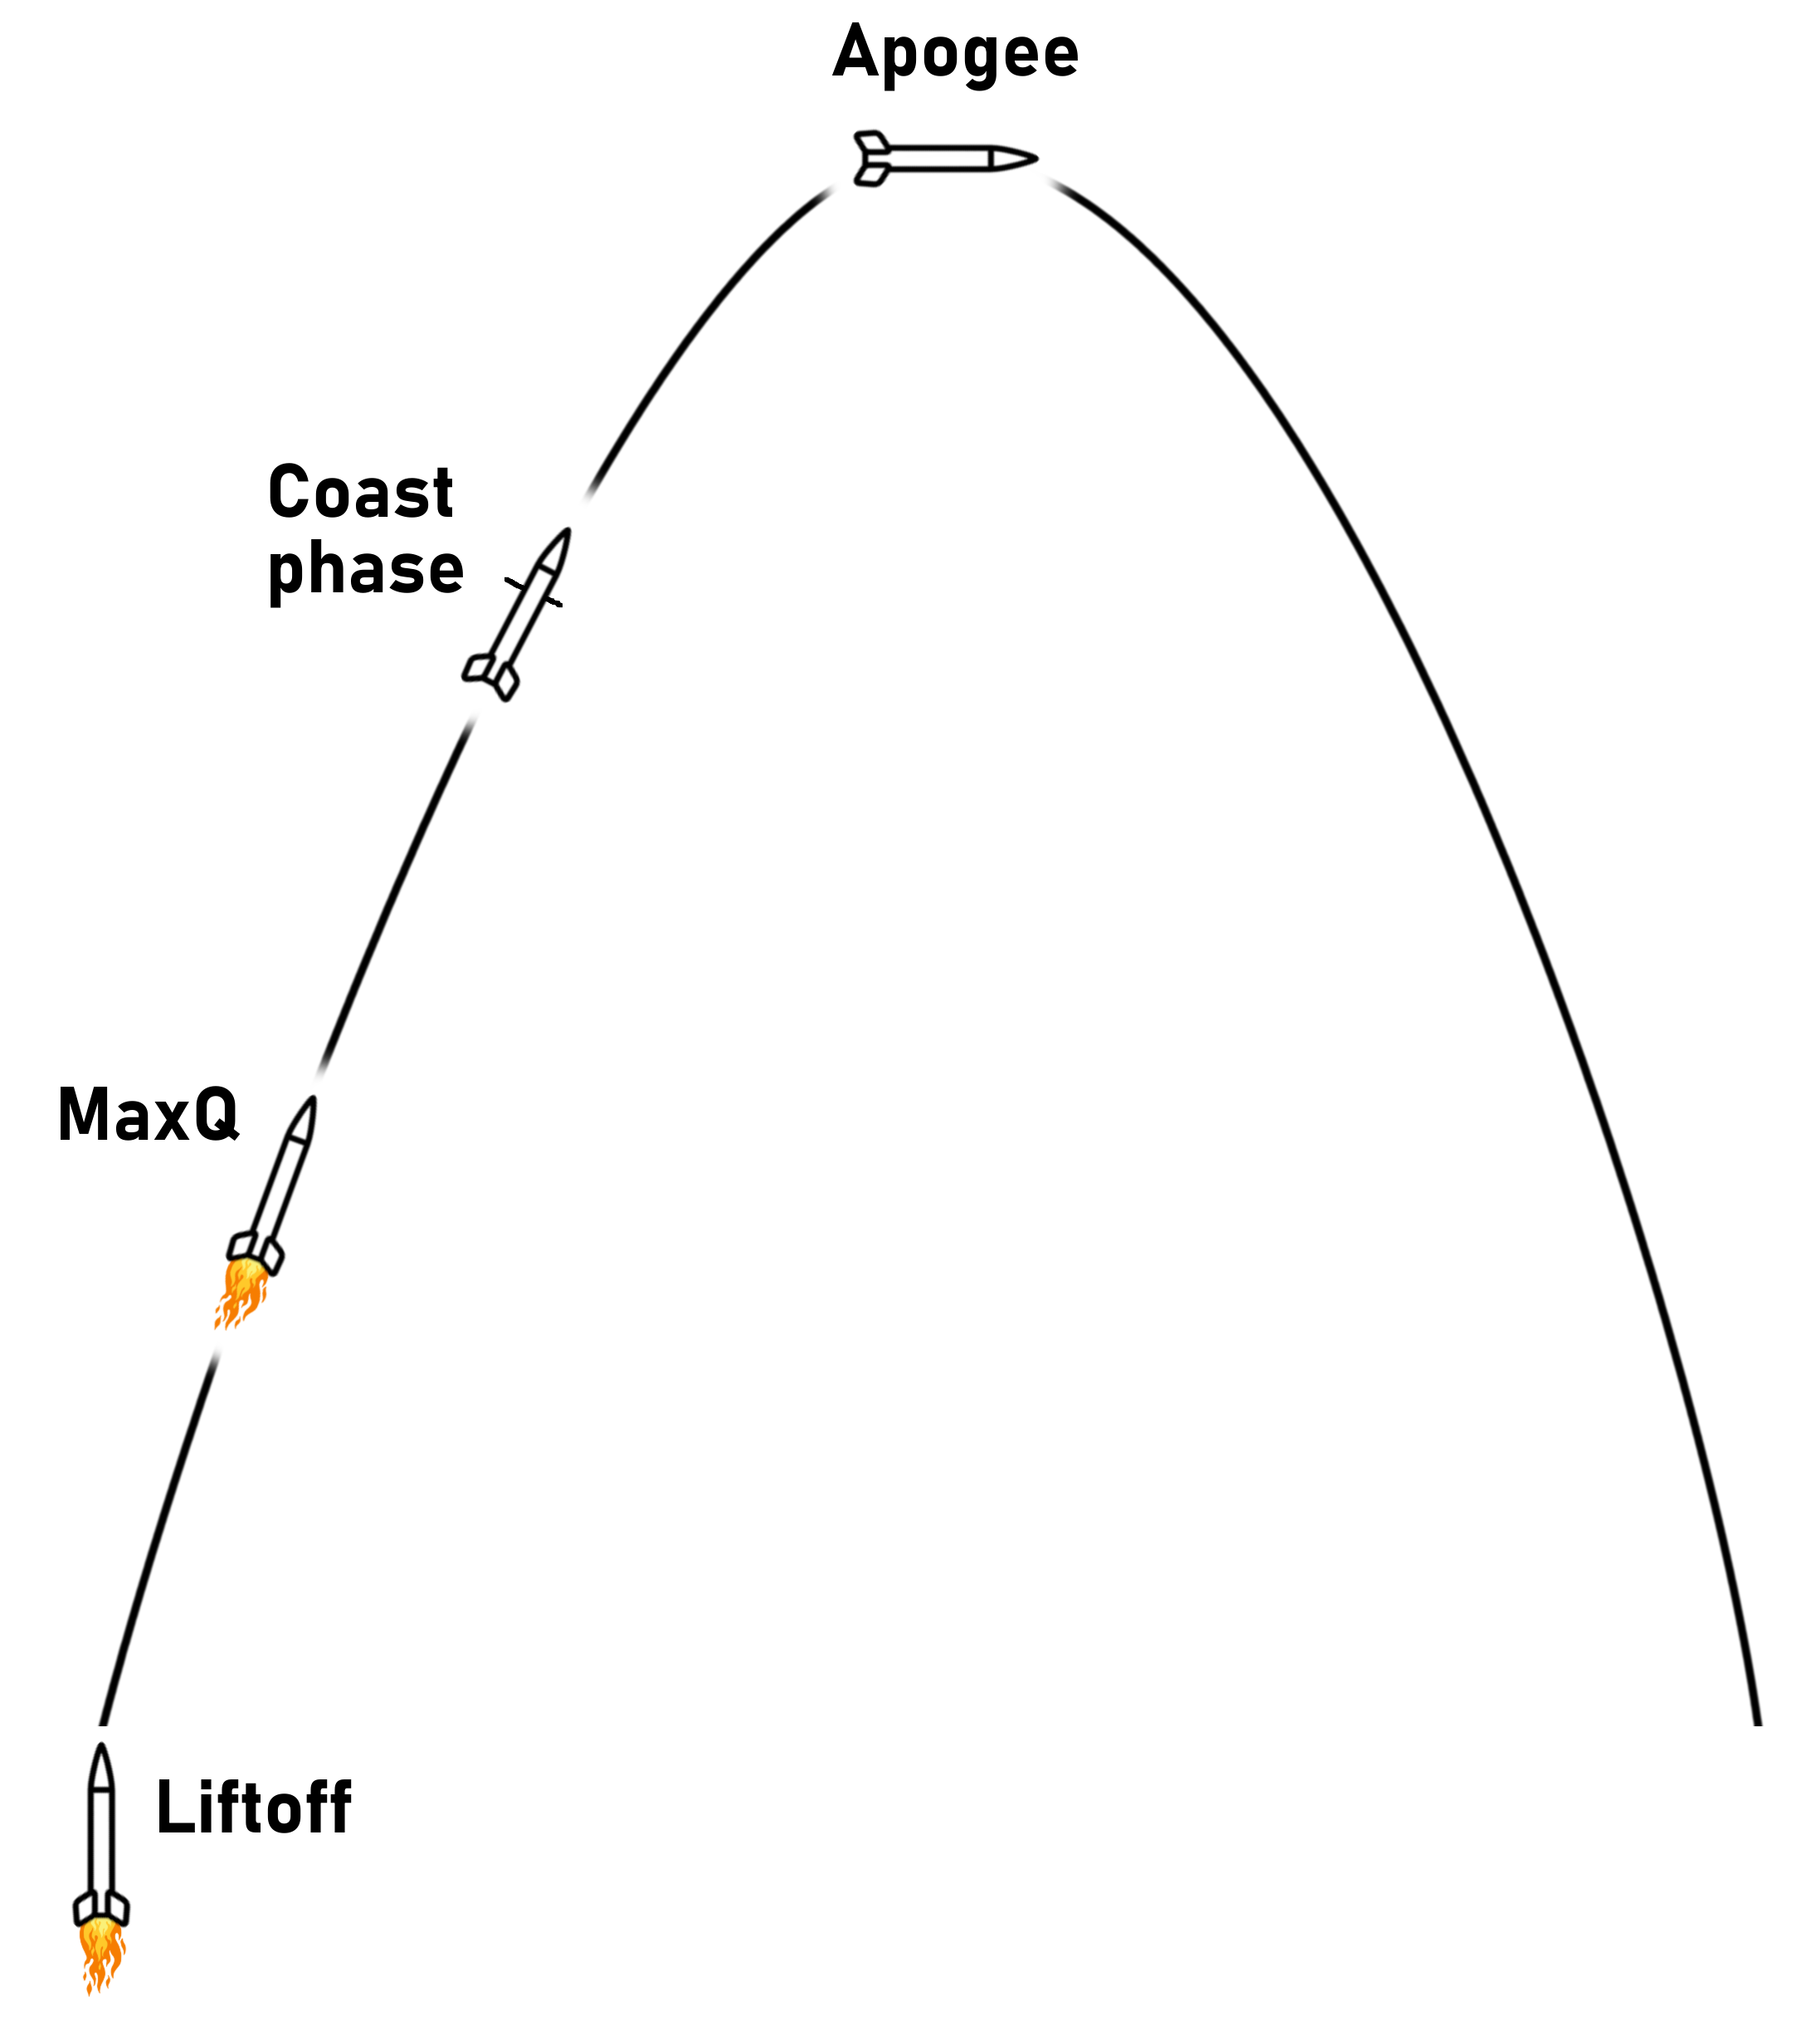
\includegraphics[height=8cm]{Trajectory.png}
	\caption[figure]{Idealized trajectory of a sounding rocket}
	\label{fig:trajectory}
\end{figure}

For this project, the following milestones are important: Liftoff, MaxQ, booster burnout, coast phase and apogee.\\
Liftoff describes - as the name implies - the moment the vehicle leaves the launch rail right after booster ignition. This is also the moment the vehicle experiences the highest amount of g-forces. This is especially important as amateur rockets usually have a very high thrust-to-weight ratio (a lot of upwards pushing force and relatively low weight). This leads to a large jolt which is especially tough on the components. \\
Shortly after liftoff, "MaxQ" or "maximum dynamic pressure" is reached. This is the maximum aerodynamical force the vehicle will face during flight, which is also related to the mechanical stress the vehicle experiences. This stress is caused by the aerodynamical forces creating bending moments on the rocket. \\
Booster burnout refers to the moment after the booster, more specifically the motor, has burned out almost entirely. Most of the time, there is a small flame coming out of the booster after burnout when it continues to burn residual propellant. The thrust of this is negligibly small. Booster burnout specifically describes the moment the booster loses the majority of it's thrust.\\
Coast phase is the time between booster burnout and apogee. This phase can be used to easily influence the flight path of the rocket. This is because during this part of the ascent, the vehicle is only subject to gravity and aerodynamical forces and not dependant on more or less random thrust of a solid motor. This makes the system highly deterministic and easily predictable. This presents the perfect opportunity for aerodynamical control\\
Apogee is the control setpoint of EAGLE. It describes the peak of flight or the highest altitude the rocket will reach. At apogee, the vertical velocity reaches $0\,\frac{\text{m}}{\text{s}}$ and the rocket begins a free fall. This usually results in the deployment of the parachute or in this case stop the operations of the airbrakes.

\section{Common airbrake designs}
A lot of student teams use a caomparable design for their airbrakes. Similarly to EAGLE, common airbeak designs use a central motor to actuate all control surfaces symmetrically. It extends control surfaces by sliding it along a guide rail. Since the motion of the control surfaces is perpendicular to the rocket's flight path and therefore airflow, the change of the cross-sectional area becomes independent of angles, which makes it both simpler, more reliable and easier to calculate.

\section{Basics of aerodynamics}
The stability of the most sounding-rockets (sub-orbital rockets) stems from their aerodynamical properties which is mostly dictated by their fin and nose cone design. This is because they disturb the airflow and therefore create acting aerodynamical forces that can make the rocket spin. However, these properties can also be used for steering or braking the rocket during flight using drag created by control surfaces (so called flaps).

\subsection{Drag} 
The working principle of airbrakes is aerodynamical drag. Drag is usually referred to as the force of resistance that a body encounters whilst moving to a (non-vacuum) medium. Drag occurs when the airflow is redirected upon hitting the surface of a body (here: a rocket). This leads to a change of speed and therefore pressure on said surface which leads to a decelerating force as seen below (Fig. \ref{fig:drag}):

\newpage

	\begin{figure}[!h]
		\centering
		\captionsetup{font=footnotesize}
		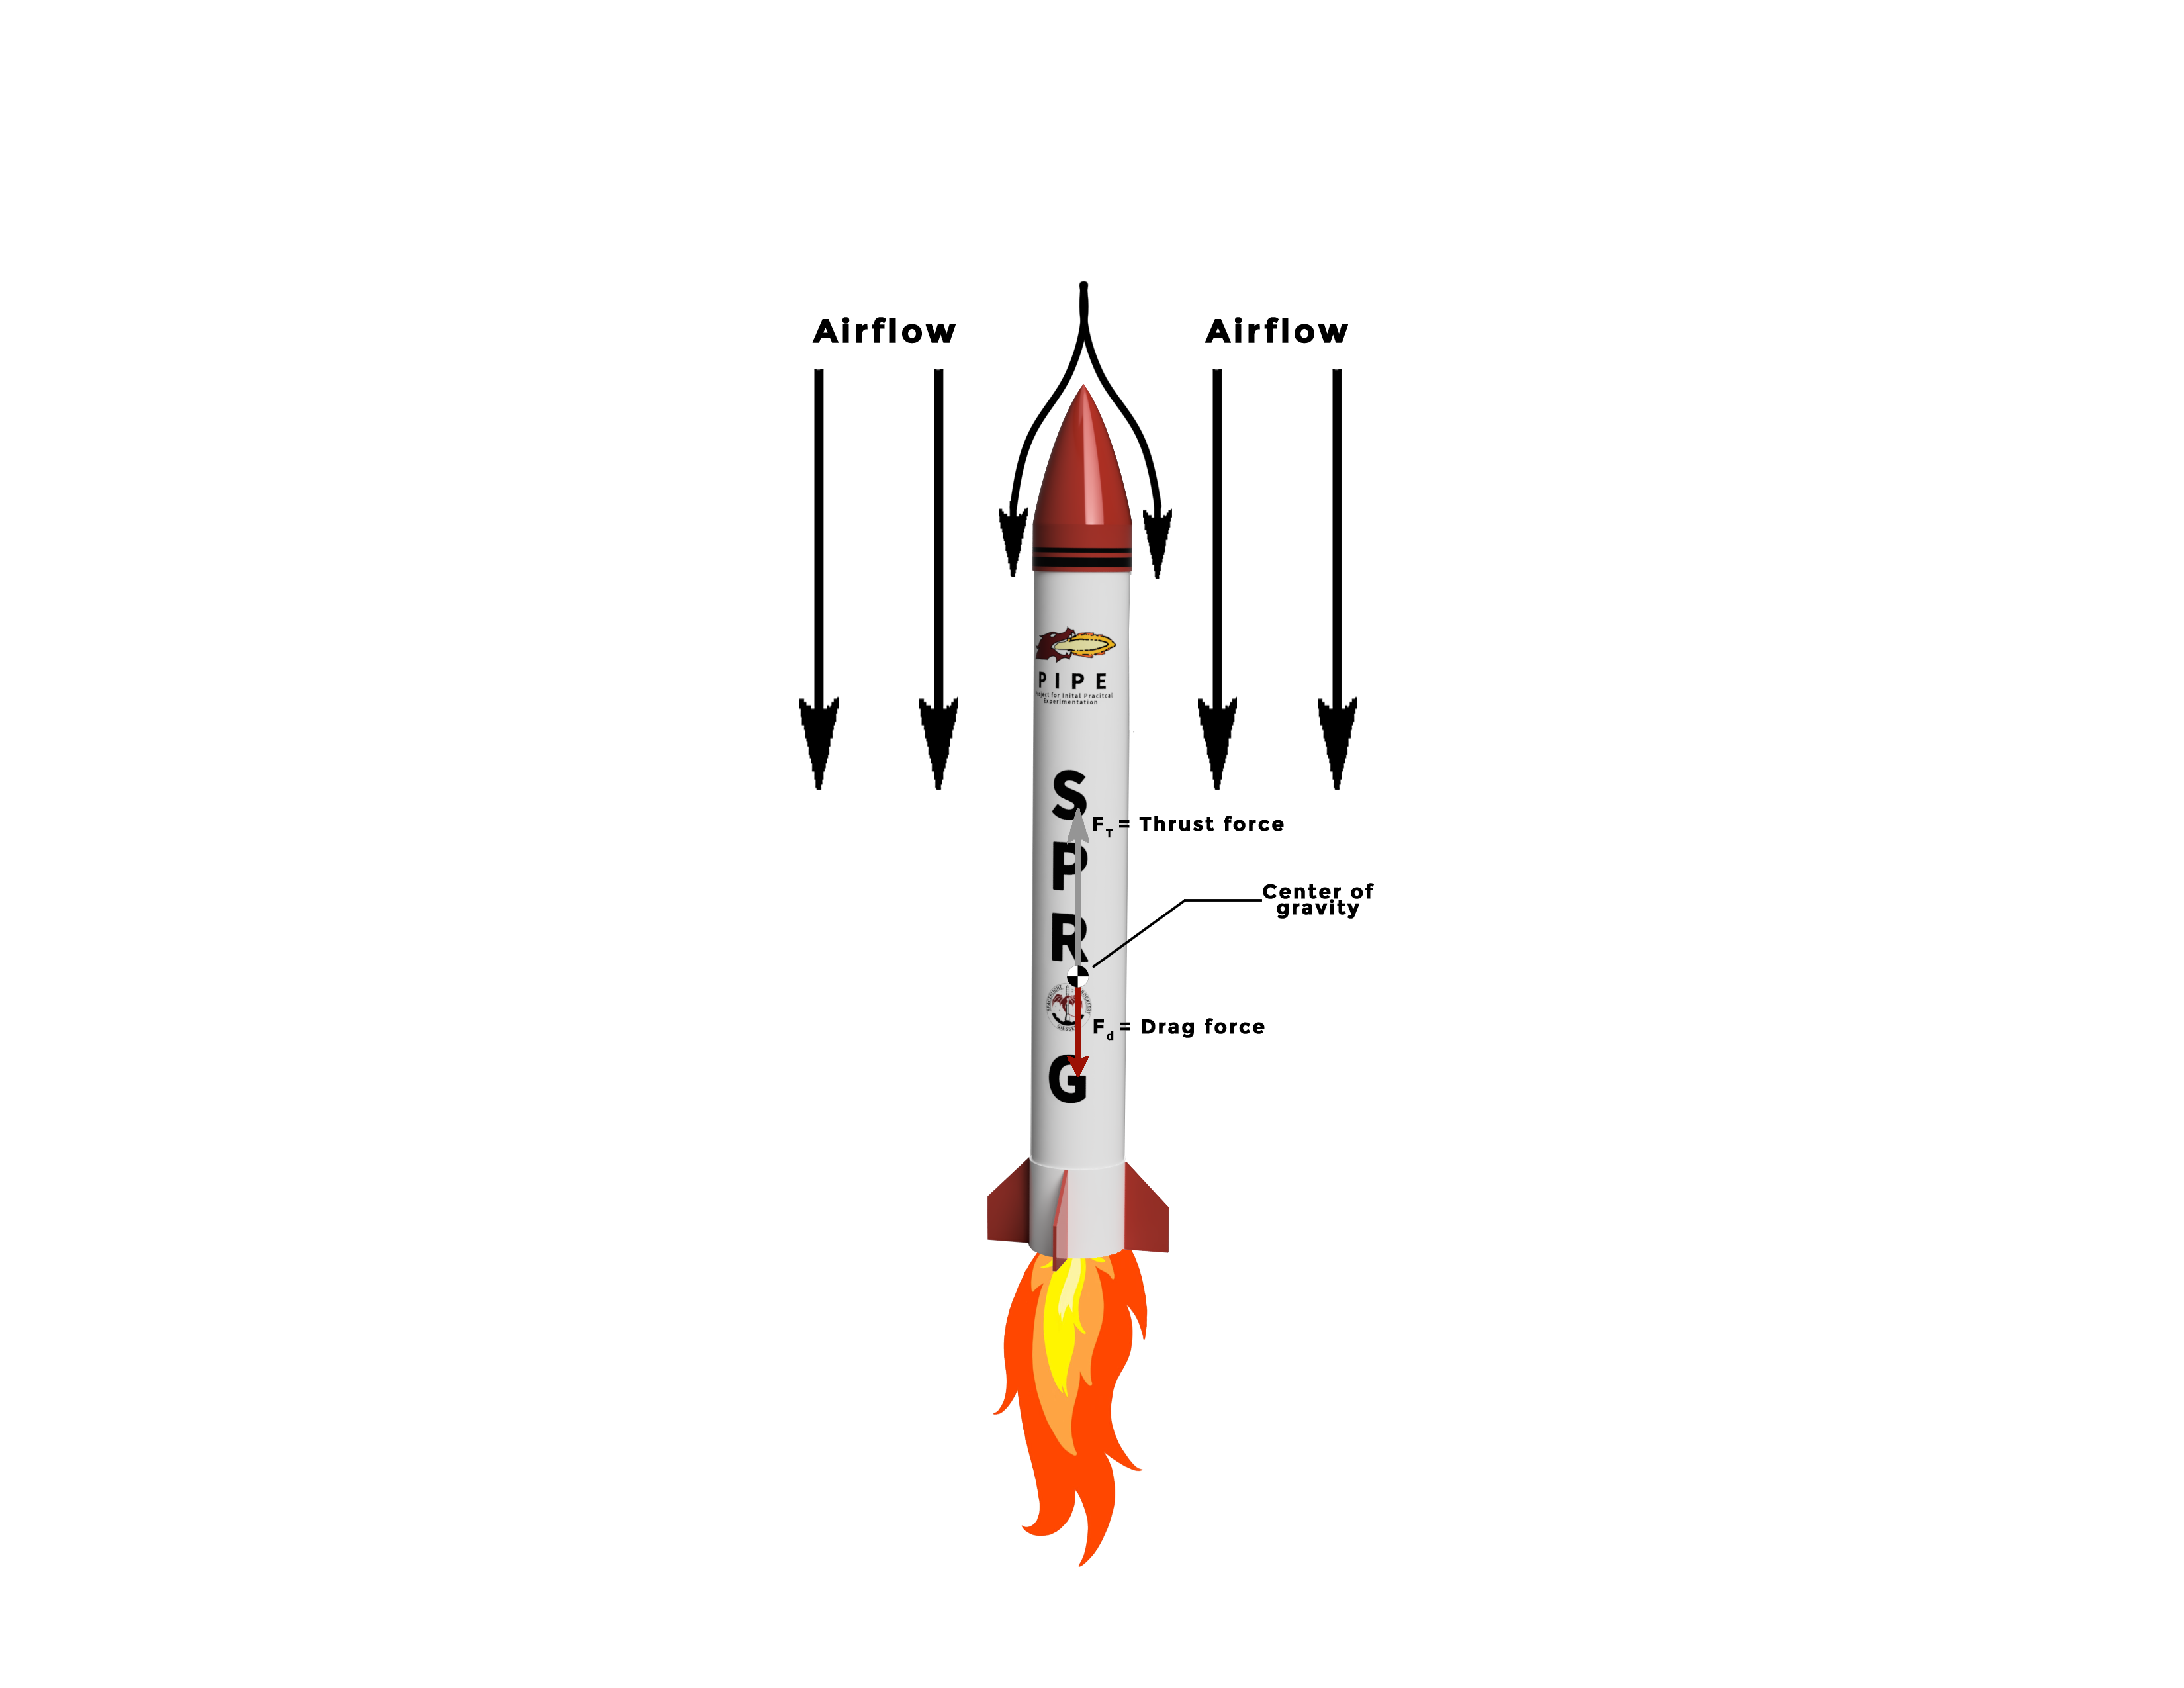
\includegraphics[height=13cm]{Aerodynamcal drag.png}
		\caption[figure]{Aerodynamical drag on a rocket during thrust phase}
		\label{fig:drag}
	\end{figure}
	
The drag that a rocket experiences is dependent on mutliple factors. A major factor is the shape of the nose cone as it is the surface that "pierces'' through the air. It "guids'' the airflow around the rocket as opposed to bringing it to an abrupt stop. This leads to a smaller rediraction of air molecules and therefore a smaller drag force.\\
Another major factor for drag is the cross-sectional area that is attacked by the airflow. The drag any body experiences due to its cross-sectional area can be calculated by the following formula:

\begin{figure}[!ht]
	\captionsetup{font=footnotesize}
	\begin{equation}
		F_\textlatin{d} = \frac{1}{2} \cdot A \cdot c_\textlatin{w} \cdot \rho_\textlatin{Air} \cdot v^2
		\label{eqn:drag}
	\end{equation}
	\caption[equation]{$A$: Cross-sectional area, $c_\textlatin{w}$: Air resistance coefficient, $\rho_\textlatin{Air}$: Air density, $v$: Airspeed} 
\end{figure}
	
\noindent Under the assumption that air density and air resistance coefficient are constant (suitable for simple expenation) equation \ref{eqn:drag} shows a proportional dependency of the cross-sectional area and a quadratic dependency of the airspeed. Airbrakes utilize the area dependency by changing the cross-sectional area $A$ of the rocket by extending control surfaces which therefore proportionally change the drag which the rocket experiences. This would have an effect on the air resistance coefficient, but this will be ignored in the scope of this project, because all calculations done within the scop of this project only serve as an estimation and not an accurate quantitative model.\\

\subsection{Aeordynamical stability}
Aeordynamical stability (stable referring to not flipping over or steering off course) of a sounding rocket is important because it does not have any active counter steering measures in case of flight path instabilities such as thrust vetor control (often seen in orbital class rockets). To understand stability we first have to understand two concepts regarding acting forces: Center of mass also known as the center of gravity (CG) and center of pressure (CP).\\
The CG is the "average mass" of a rocket summarized in a single point. It is also where the gravity forces acts. The CP is a concept in fluid dynamics which describes the point on a body where a single acting force can describe the entire effect on an acting pressure difference (i.e. drag/lift forces).\\
In order to guarantee a stable rocket the CP must be located behind the CG. This is because the acting fluid-dynamical (equivalent to aerodynamical) forces act on the CP which causes a torque and therefore a rotation on the rocket. This rotation changes the angle of attack (AoA) - angle under which the air hits the surface - of the airflow in regards to its fins. If the CP is located behind the CG, the changed AoA will result in a resisting lift force on the fins which will in turn rotate the rocket back to its original rotation. If the CP is sitting in front of the CG the created lift from the fins and the applied torque on the rocket no longer cancel each other out, but add to each other which results in a bigger angular velocity and aerodynamical control loss. This is shown in figure \ref{fig:stability}:

\begin{center}
	\captionsetup{font=footnotesize}
	\begin{figure}[!h]
		\subfigure{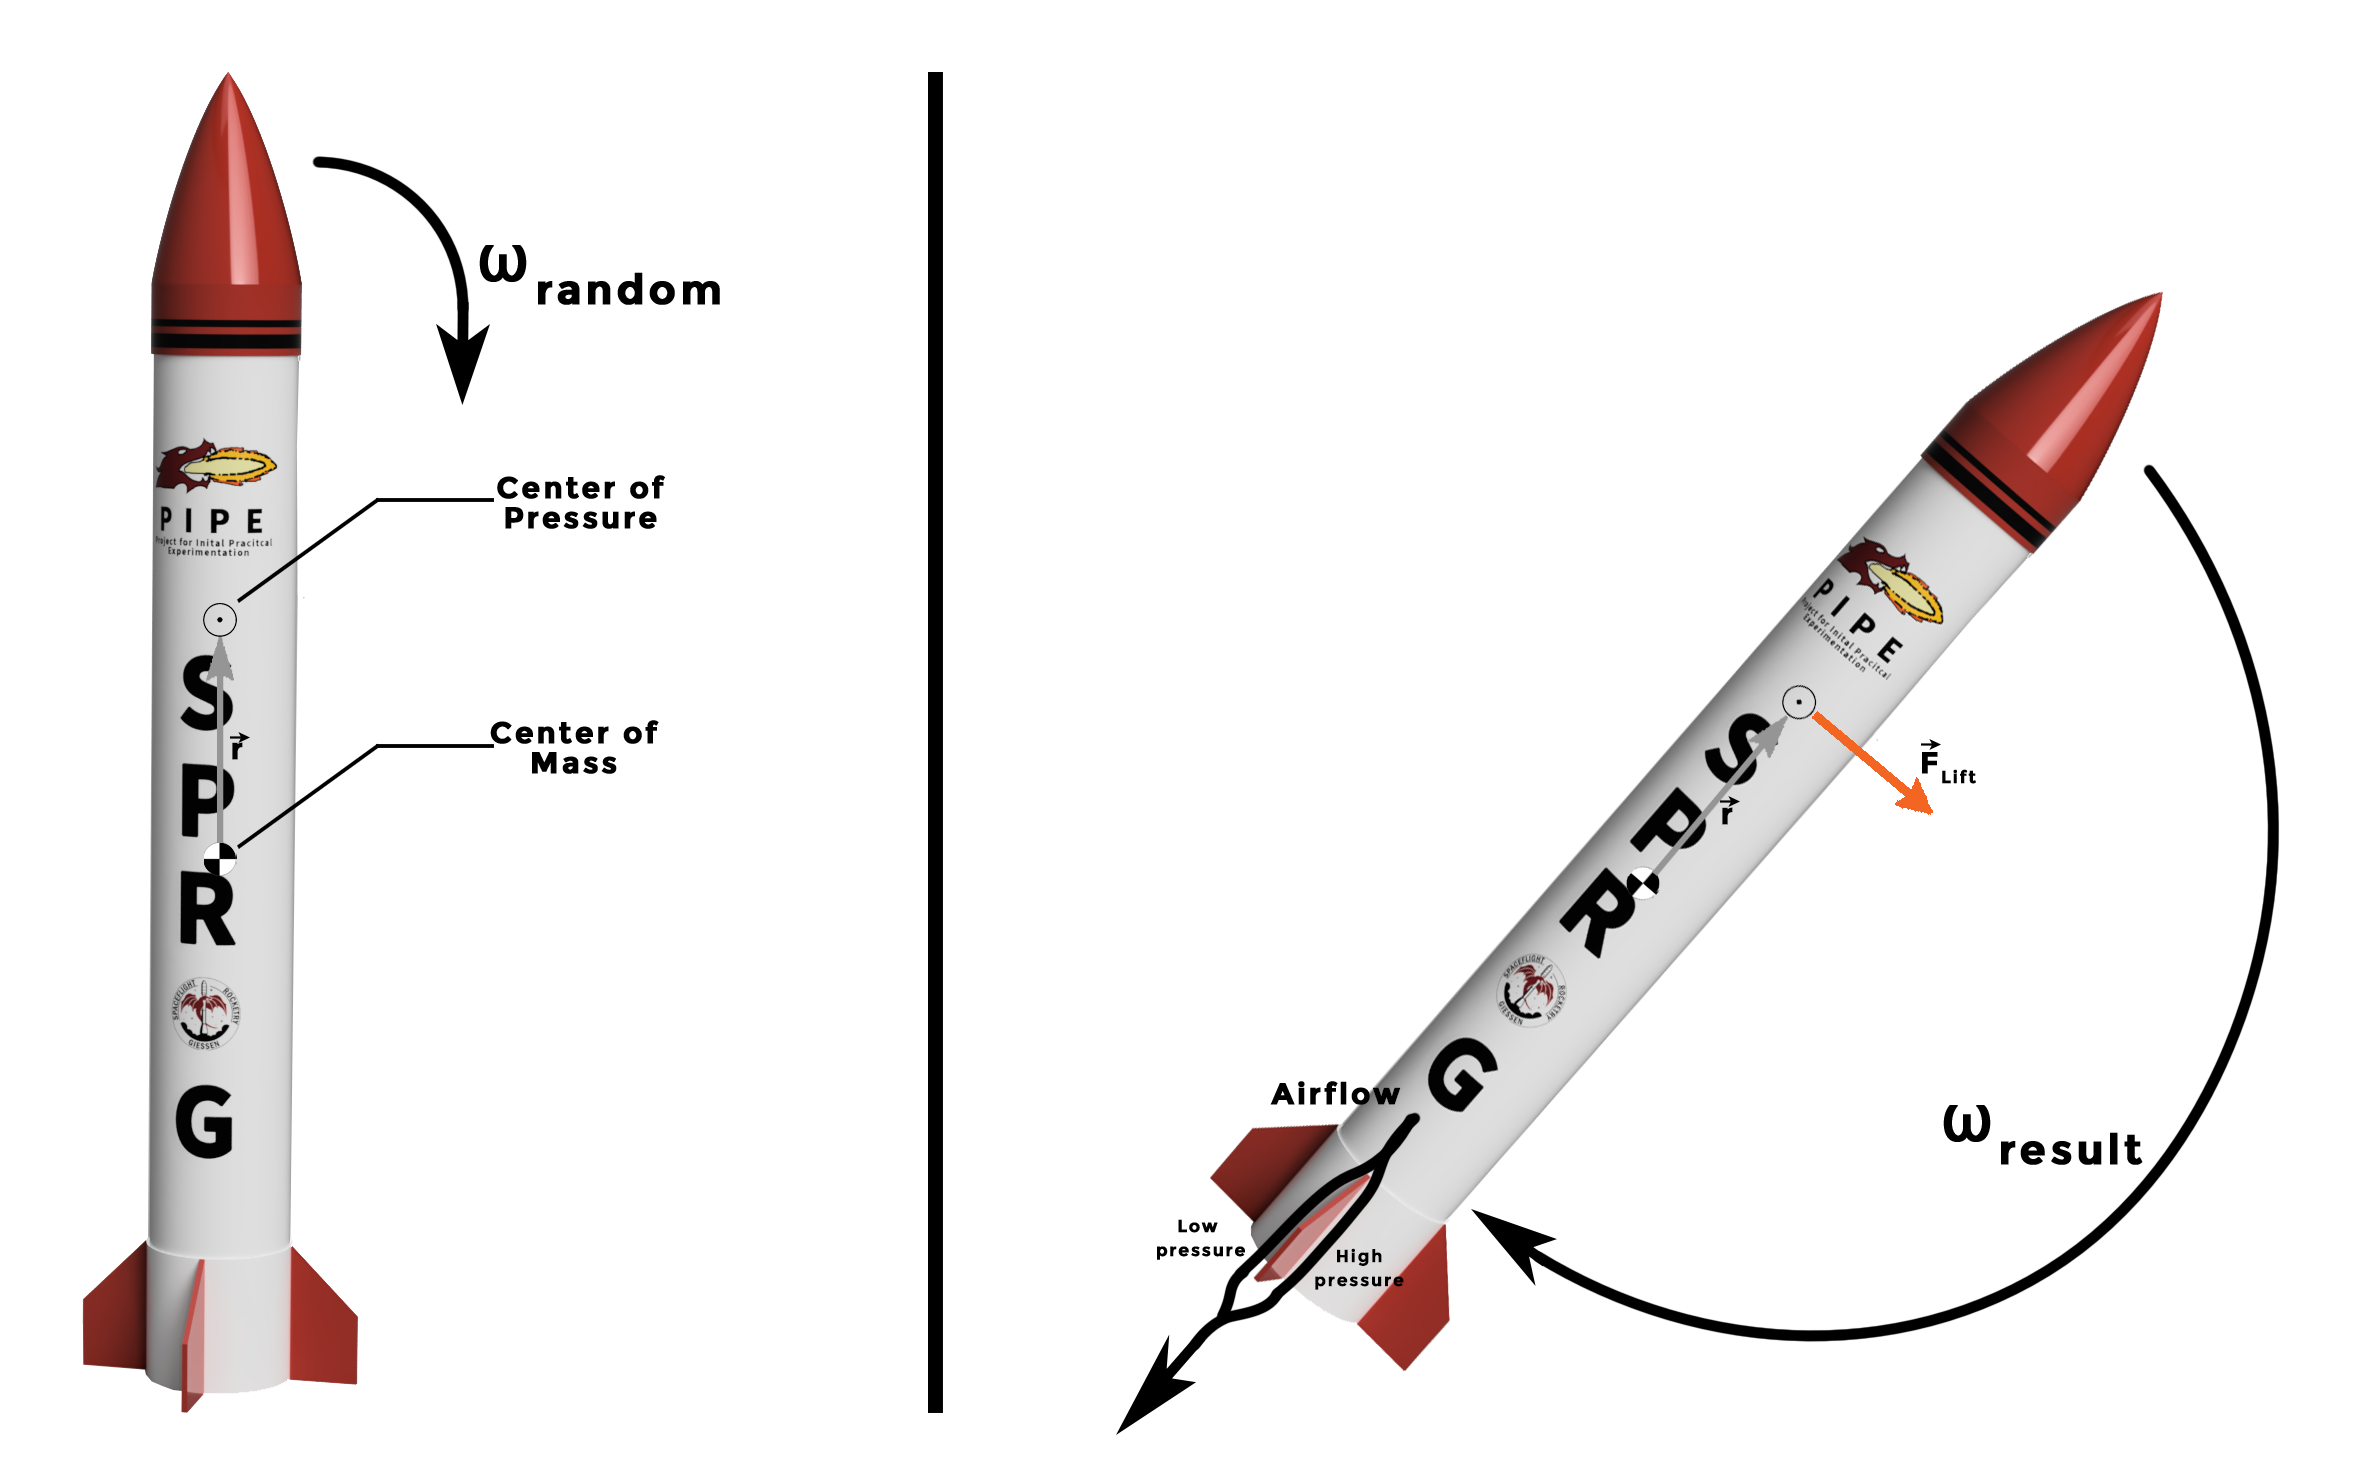
\includegraphics[height = 5cm]{Stability 1.png}}
		\hspace{1cm}
		\subfigure{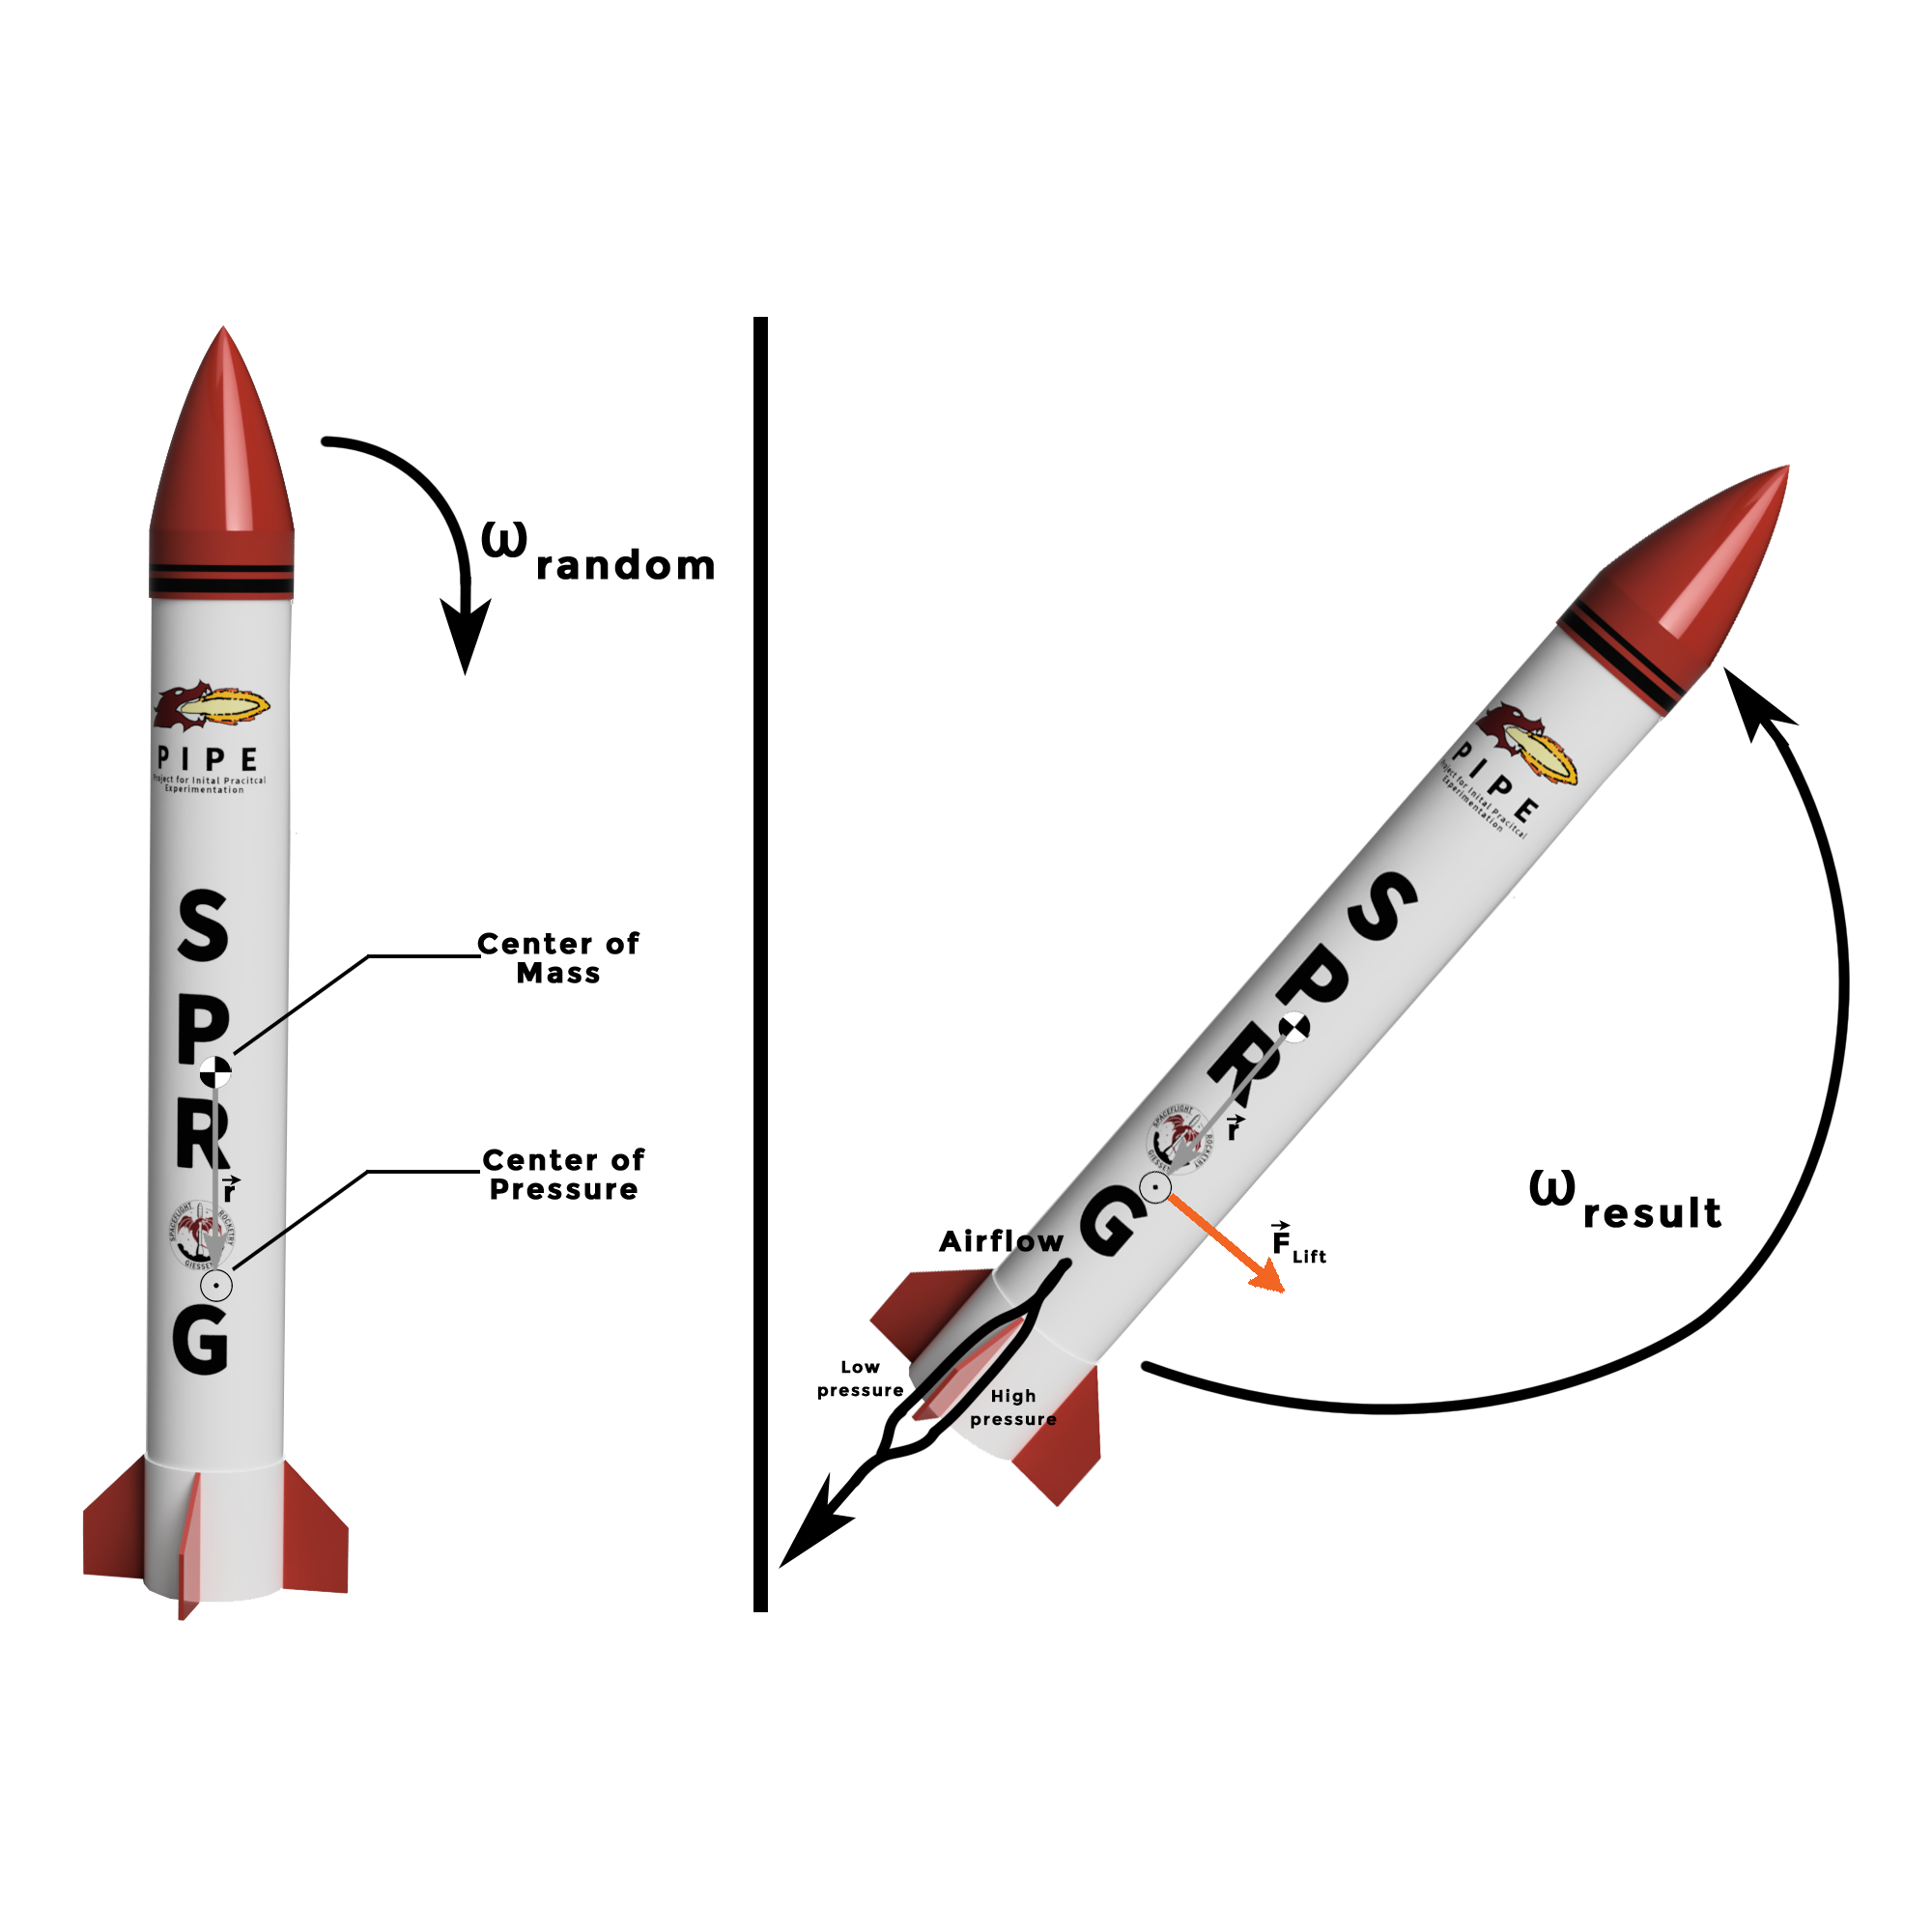
\includegraphics[height = 5.5cm]{Stability 2.png}}
		\label{fig:stability}
		\caption[figure]{Left: CP in front of CG, Right: CP behind CG}
	\end{figure}
\end{center}

The CP usually follows the direction of the aerodynamical surfaces (i.e. the fins), meaning that fins towards the nose of the rocket would result in the CP moving towards the nose as well. The Figure \ref{fig:stability} shows what would happen if the CP moves in front of the CG and implies why fins are usually located at the back of a rocket. 

\begin{figure}[!h]
	\centering
	\captionsetup{font=footnotesize}
	\includegraphics[height=7cm]{airbrake design.png}
	\caption[figure]{Commonly used airbrake design \cite{Airbrakes}}
	\label{fig:airbrake}
\end{figure}	

\noindent For EGALE, it was decided to go for a more complex approach to increase the learning opportunity by working closer with to proven designs commonly used in the aerospace industry, e.g. grid fins.

\subsection{Control authority}
Control authority is a term used in guidance, navigation and control (GNC) to describe the amount of influence on a rocket's trajectory. This can either mean that there is a large thrust-to-weight ratio, meaning that the inputs of thrust-vector-controls will result in a bigger torque on the vehicle and will therefore turn the rocket more than with a lower thrust-to-weight ratio.\\
In the case of aerodynamical control, a higher control authority can be achieved by bigger acting aerodynamical forces. As seen in equation \ref{eqn:drag}, the drag force is quadratically dependent on the velocity $v$. This means that the rocket experiences bigger forces when going as quickly as possible (under the assumption that other parameters are constant). During MaxQ, these aerodynamical forces are the highest during the entire ascent phase, which also gives us the biggest control authority. However, it does not make sense to break while the rocket is still accelerating (during boost phase at MaxQ) because there is too much variance in an apogee estimation during that time because of the booster own variance. \\
During the coast phase, the rocket slowly loses its velocity and therefore its control authority because it is being descelerated by gravity. If it is required to create major corrections to the trajectory, it is important to use as much control authority as possible i.e. extend flaps right after booster burnout, if necessary. This not only gives more time to react, but also gives more room for corrections if the controller has overshot its target by breaking too much (which can happen with common PID controllers).

\newpage

\section{Load estimation}
To estimate whether or not a part is mechanically sound, the load on said part needs to first be estimated through some calculations. When it comes to loads there are two parameters we care about: Attacking forces and torque.\\
The acting forces on a rocket during the coast phase (after booster burnout and before apogee) are the before-mentioned drag/lift forces as well as gravity. Gravity acts on the center of mass, whilst drag and lift attack on the so called center of pressure.\\
The acting torque on the fins $\vec{M}$ can be calculated by taking it's lever arm $\vec{r}$ and the acting force $\vec{F}$ into consideration:

\begin{subequations}
	\begin{align}
		\vec{M} &= \vec{r} \times \vec{F} & \text{with } \vec{r} \perp \vec{F} \label{eqn:torque_vec}\\
		M &= r\cdot F
		\label{eqn:torque_lin}
	\end{align}
\end{subequations}

The torque is proportional to the absolute value of the force and the lever arm (if force vector is perpendicular to lever vector). This means that a mean to reduce load is to reduce the lever length or reduce the acting force.

\section{Common grid fins} \label{sec:Grid fins}
Common grid fin designs such as the ones that can be found on SpaceX's Falcon 9 rocket is a proven concept that has not only been validated regarding its performance, but also its reliabilty over mutliple mission cycles. These fins are commonly put on the outside wall of the airframe of the rocket and are locked in position until the reentry of the vehicle on descent (as seen in the fig. \ref{fig:F9 grid fin}).

\begin{figure}[!h]
	\centering
	\captionsetup{font=footnotesize}
	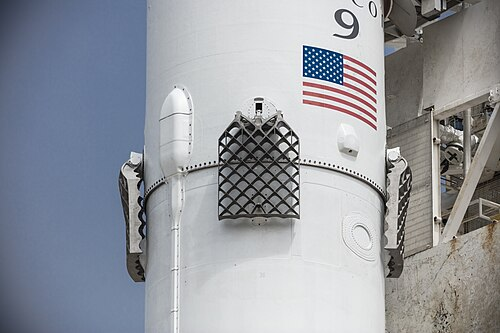
\includegraphics[height = 7cm]{SpaceX grid fins.jpg}
	\caption[figure]{Falcon 9 grid fins - Iridium 2 mission \cite{Falcon_9_grid_fins}}
	\label{fig:F9 grid fins}
\end{figure}

These have a resting angle i.e. the resting position under normal flight conditions of 0° towards the airframe and a 90° angle upon actuation. They serve the purpose of steering the rocket towards the landing zone upon reentry and whilst the engines are not performing a landing/reentry maneuver. For that they use an extra degree of freedom (DoF) on top of the outward motion i.e. they can turn around their own axis. However, this "extra" DoF is not discussed further as it does not match requirements of the design described in this report.



\newpage
\chapter{Airbrake design}
The purpose of this chapter is to show the methodology used during the development of the airbrake system and highlight issues and difficulties that were encountered and considered in later iterations of the airbrakes.\\
Furthermore, it serves as an introduction to the first iteration of airbrakes to understand important findings in regards to further development.

\section{Methodology}
Typically, issues  that were encountered during the development of EAGLE could be categorized into different groups, such as mechanical robustness, aerodynamical properties and (reliable) producibilty. The latter being one of the most important aspects and reason for a majority of changes.\\
Said issues could be identified through a 3d-printed full-scale model of design iterations, which may unveal flaws in regards to said categories.

\section{Mechanical robustness}
To understand mechanical issues, they first need to be broken down further in regards to the following sub-categories: \textit{Load-bearing structure or mechanism}. The first referring to parts that carry a large amount of the expected loads during flight and the latter referring to parts directly involved in the actuation mechanism of the flaps.\\
There are certain fundamental aspects that need to be considered for load-bearing parts such as the question whether a part can actually sustain the loads during flight or if it can be made stronger without sacrificing performance. \\
The approach to these issues was to estimate which parts would see a majority of the load and estimate the load through simplified calculations and verify these values during testing.

\section{Aerodynamical properties}
The most important aerodynamical property is stability as it is the only thing keeping the rocket from spinning out of control which could lead to a loss of the vehicle or worse the rocket moving uncontrollably towards the ground, which is why the stability of the rocket must always be retained even when deploying the airbrakes.\\
This can be ensured by simulating the rocket in a rocket simulation program such as the open-source tool called "OpenRocket" both with undeployed and fully deployed flaps as those edge cases will result in the biggest movement of the CP. Afterwards smaller fin-sizes were evaluated to fine-tune the CP to stay inbetween acceptable margins of the stability margin (between 1.5 and 3 caliber).

\section{Producibilty}
A large factor to keep in mind when designing parts of assemblies is the producibilty and maintanibility. The first includes both the complexity of manufacturing and segment cost (cost of all parts in relations to the airbrakes). The aim is to keep both to a minimum. Maintanibility refers to how easy or hard it is to replace or repair certain parts. This is important to ensure the longevity of a part and guarantee that emergency repairs can be done quickly and without high costs. This can be achieved by basing the design off of COTS components and reducing the amount of custom parts as COTS parts are usually cheaper and can be bought in bulk whilst custom parts require specialized tools and are one of a kind parts that can take days or weeks to have manufactured and delivered. Ease of repairability can be tested by manufacturing prototypes from 3D-printing.



\chapter{Airbrakes v1\footnote{This design iteration was developed together with Vincent Uebel}}

This chapter deals with the first iteration of the airbrake design to outline underlying issues regarding the before mentioned aspects of the desing process, while also giving insights into the decision making.

\section{Concept}
The first iteration relied on the working principle of a piston in an engine, where you have guiding elements for a pushing rod which is freely connected to a connecting rod which itself is freely connected to a servo-cross on the servo-gear. The pushing rod would then push out the flap which itself is, at its core, just a cutout of the body tube as seen in fig. \ref{fig:airbrake v1_parts}.

\begin{figure}[!h]
	\centering
	\captionsetup{font=footnotesize}
	\includegraphics[height=7cm]{airbrakes v1 - parts.png}
	\caption[figure]{(1): Guiding elements, (2): Pushing rod, (3) Connecting rod, (4): Servo-cross, (5): Servo-gear, \hspace{1cm}(6): Flap (PLATZHALTER -> NOCH BESSERES BILD MACHEN)}
	\label{fig:airbrake v1_parts}
\end{figure}

BILD FÜR PLEUEL

The mechanism and servo are held in place by a custom inner structure, which is glued to the inside of the body tube. The guiding rails is then fixed onto the inner-structure. The flaps are loosly connected to the pushing-rod and the hinges are also attached onto the inner wall of the body tube. With this design, the flaps would have a maximum deployment angle of approx. 15°.\\
Larger parts are designed to be 3D-printable, meaning they do not rely on tight tolerances and are purposefully bulky to be able to sustain the loads that these parts would face in supersonic flight. This was done to reduce overall cost by avoiding metal manufacturing of large custom parts.

\section{Discovered issues}
A first prototype was manufactured using only 3D-printing. The purpose of this was to verify the basic working principle of the mechanism and discover issues with production. The point of this section is to  highlight these issues.

\subsection{Mechanical robustness}
One major issue that was discovered after printing out the parts for the first time was that the parts are severly undersized to bear any kind of load, even when made out of metal. In retrospect, this was most likely caused by a false sense of scale in the 3D-model, which is a common mistake in CAD-design as parts appear bigger on screen. Furthermore, all 3D-printed parts, except for the large inner structure have not been of high enough quality leading to imperfections and inconsistencies in holes, which had to be drilled open to allow for the pushing rods to smoothly slide through the guide rails or to allow the hinge-bar to freely turn in the hinge.
On top of that, the flaps would require to cut out large portions of the body tube, which would severely weaken the structural intergrity of the carbon fibres because the carbon fibre weave is cut open. With the inner structure glued to the inside of said carbon fibre tube, all loads would be directly transfered to the already weakened tube, which makes it the major load bearing structure. This would most likely lead to a mechanical failure at supersonic speeds.
The mechanism itself however, has proven itself to work, delivering the desired symmetrical behaviour.

\subsection{Aerodynamical properties}
The expected range of drag increase can be calculated using equation \ref{eqn:drag}. A maximum flap deployment angle of approximately 15° leads to a marginal increase in cross-sectional area and therefore to a relatively small increase of drag. This would allow for very precise altitude control, but not for a big influence on the final trajectory. However, solid rocket motors have slight variations in their behaviour between each motor, even when they are of the same specifications. This is because of its inner geometry which is varying with every cast motor. This means that the motor could overperform and therefore overshoot the simulated alltitude, it could underperform and not reach the simulated altitude or it could perform nominally and reach the simulated altitude precisely. There is, however, no way to determine a motor's performance before firing it, meaning that the airbrakes would need to cover a broad range of trajectory corrections to perform accurate altitude control. To achieve this with the current design, the size of the flaps would need to significantly increase, which would lead to bigger tube cutouts and therefore a weaker structure overall. That is why a sufficient sizing of these flaps was not possible with this design.

\subsection{Producibilty}
Producability has proven itself difficult with the prototype as it required to glue a lot of small parts by hand which is inconsistent and inaccurate. It is also required to assemble parts outside of the body tube. The hingeplates need to be put on the hinge-bar before, glueing them in. This also means that you have to disassemble multiple parts, if only one part broke. This proves difficult if parts are either glued or epoxied in place as they stick to the inside of the body tube quite well. This would most certainly damage the inside of the rocket or one of the components that has to be taken off just to repair another part. Additionally, it is possible to have glue reach into the mechanism during the installation of parts rendering all kind of movement impossible. Furthermore, all parts of that design are custom parts meaning no parts could be bought off the shelf and would need to be produced by us or an external contractor, meaning spontaneous repairs are unfeasible. On the other hand, with major parts being 3D-printable, it would significantly cut down cost and weight of major components, which is a major driving factor in student rocketry. Overall, the procducability was proven to be too unreliabel whilst the cost efficincies do not make up for the unefficiencies in other factors.

\chapter{Airbrakes v2}
Due to the above mentioned reasons it was decided to change the basis of the design and try to work closer to industrially proven ways for flap design. It was also decided to design around more COTS parts and parts, which can easibly be produced in bulk. All of these decisions and changes will be highlighted in this chaper.

\section{Concept}
As described in chapter \ref{sec:Grid fins}, the range of motion of the Falcon 9's grid fins match the motion requirements of fins described in this report and have heavily influenced the working principle of this iteration of airbrakes.
The second iteration is mainly based on mechanical gears as they can be sized based on mechanical load calculations using different gear ratios to reduce the experienced torque on the servo motor. Furthermore, the flaps would no longer sit flush against the outside of the body tube of the rocket, but rather sit outside of it when unactuated, as seen in fig. \ref{fig:airbrake v2 - closed}\footnote{Load bearing structure unfinished as they will be connected to the interstage rings, which have not been designed yet}\footnote{Ball bearings which hold the driveshaft are not modelled in the CAD model as manufacturer did not provide a 3D-model}:

	\begin{figure}[!h]
		\centering
		\captionsetup{font=footnotesize}
		\subfigure[(Red): Aero cover,  (Yellow/Green): Screw adapter, (Blue) Load bearing structure, (White - outside): Fins, (White - middle): Gearbox-structure, (Grey/Yellow): 4-way mitter gear (gearbox) + driveshaft]{\includegraphics[width=0.42\textwidth]{airbrakes v2 - closed.png}}
		\hfill
		\subfigure[Sectioned view of airbrake v2]{\includegraphics[width=0.51\textwidth]{airbrakes v2 - closed_section.png}}
		\caption{airbrakes v2 unactuated}
		\label{fig:airbrake v2 - closed}
	\end{figure}

\newpage

The load bearing structure carries most of the mechanical load. In order to reduce strain on the carbon tube, they will be directly attached to the interstage rings that connect different rocket segments. The screw adapters are slid in between the load bearing structure and the airframe and then put into place by screwing into the aero covers on the outside of the airframe. The aero covers serve the purpose on guiding the air over the cutout created by the fins to turbulence and therefore unpredictability and drag. The gearbox-structure is a jig to help allign the ball bearings, which are holding the driveshaft in position. It is directly attached to the load bearing structure, but only carries the weight of the ball bearings. The flaps are inspired by common grid fins known from reusable orbital class rockets such as SpaceX's Falcon$\,9$. The surface area of the flaps are not sized according to calculations. The size will be fine tuned after the working principle of the mechanism is confirmed and accepted. \\
All screw points are at an angle of 45° to reduce strain on them. The angle distributes the acting forces to both the vertical and horizontal direction.

\subsection{Load calculations}
To adequately size the servo-motor, some assumptions of the mechanical load of the servo motor will have to be made, so that the motor can survive and also sustain the loads expected during flight. The load on the servo is mostly determined by the acting torque of the fins. The torque on the servo can be estimated using equations \ref{eqn:drag} and \ref{eqn:torque}. This will allow for the biggest sustainibility to high forces and will therefore allow for more control authority.\\
For this example calculation the worst-case scenario was assumed. This means that all parameters are assumed to be constant. This assumption can be made for the worst-case scenario, because the air-density lowers in higher altitudes which in turn lowers the drag-coefficient. Furthermore, it was also only calculated for full flap deplyoment as this will deliver the biggest drag on the vehicle and therefore the biggest torque. This also means that equation \ref{eqn:torque_vec} can be simplified to equation \ref{eqn:torque_lin}, since the force vector would then be perpendicular to the lever vector.\\
What matters most is to keep high control authority for as long as possible. This is why for this example only the servo motor from ,,MKS servo tech" (supplier) with the highest torque will be considered and evaluated. This will allow to deploy the flaps earlier and therefore make corrections easier. To estimate the time which can be used to actively change the flight path and the max. velocity that the servo can sustain, the following calculations can be made:

\begin{subequations}
	\begin{align}
		M &= r\cdot F & \text{with } F_\textlatin{d} = \frac{1}{2} \cdot A \cdot c_\textlatin{w} \cdot \rho_\textlatin{Air} \cdot v^2 \\
		M &= \frac{1}{2}\cdot r\cdot A \cdot c_\textlatin{w} \cdot \rho_\textlatin{Air} \cdot v^2 \\
		v_\text{max} &= \sqrt{\frac{2\cdot M_\text{max}}{r\cdot A\cdot c_\text{w}\cdot \rho_\text{Air}}} & \text{with } A = A_\text{fin} + A_\text{body} \\
		v_\text{max} &= \sqrt{\frac{2\cdot M_\text{max}}{r\cdot (A_\text{fin} + A_\text{body})\cdot c_\text{w}\cdot \rho_\text{Air}}}
		\label{eqn:vel_max}
	\end{align}
\end{subequations}

\newpage

Using the following parameters of the airbrake v2 design and equation \ref{eqn:vel_max}, we get the following results:

\begin{itemize}
	\item Lever $r$:  $0.04\,\text{m}=const.$
	\item Cross-sectional area (per fin) $A_\text{fin}$: $0.002699\,\text{m}^2=const.$
	\item Cross-sectional area (airframe) $A_\text{body}$: $0.0804096\,\text{m}^2=const.$
	\item Drag-coefficient (cylinder) $c_\text{w}$: $0.35=const.$
	\item Air density (atm) $\rho_\text{Air}$: $1.18\,\frac{\text{kg}}{\text{m}^3}=const.$
	\item Max. velocity\footnote{,,strongest" servo available in supplier's store} $M_\text{max}$: $6.668\,\text{Nm}$
\end{itemize}

\begin{align*}
	v_\text{max} &= \sqrt{\frac{2\cdot M_\text{max}}{r\cdot (A_\text{fin} + A_\text{body})\cdot c_\text{w}\cdot \rho_\text{Air}}}\\
	&= \sqrt{\frac{2\cdot 6.668\,\text{Nm}}{0.04\,\text{m}\cdot (0.002699 + 0.08041)\,\text{m}^2\cdot 0.35\cdot 1.18\,\frac{\text{kg}}{\text{m}^3}}}\\
	v_\text{max} &\approx \underline{\underline{ 89.18\,\frac{\text{m}}{\text{s}}}}
\end{align*}

WRONG VALUE\\\\

Using this velocity, it is possible to calculate the reaction time until apogee. As explained in chapter \ref{sec:traj}, apogee is the point in flight where the vehicle's vertical velocity reaches $0\,\frac{\text{m}}{\text{s}}$. Assuming an ideal and straight flight, the time to apogee $\Delta t_\text{apogee}$ and therefore the time in which the flight path can be changed can be calculated like the following:

\begin{align*}
	\Delta t_\text{apogee} &= \frac{v_\text{max}}{g} & \text{with } g = 9.81\,\frac{\text{m}}{\text{s}^2}\\
	&= \frac{89.18\,\frac{\text{m}}{\text{s}}}{9.81\,\frac{\text{m}}{\text{s}^2}} \\
	\Delta t_\text{apogee} &= \underline{\underline{9.09\,\text{s}}}
\end{align*}

WRONG VALUE \\\\

\newpage

\section{Mechanical robustness}
This chapter shows the improvements that came with this iteration, but also highlight some persisting mechanical as well as newly arisen issues.

\subsection{Improvements}
In comparison to v1, this iteration has signigicantly reduced the body tube cutouts. For this design, only the range of motion of the flap arm needs to be cutout. This reduces the cut out area by more than half, significantly lowering the mechanical effects on the body tube. On top of that, the components no longer rely on friction or glue to stay in position. Every component is secured with screws which are tilted at a 45° angle to reduce shearing loads on the screws.\\

\subsection{Issues}
The load bearing structure features a thin wall strength, which generally does not fit as a load bearing structure. The thin wall strength could snap under high lateral G-forces or strong vibrations. This would mean that the structure fails its sole purpose, which is not acceptable for flight.\\
The amount of torque on the servo is also higher than expected, which resulted in a much lower time to apogee and therefore less control authority. 

\section{Aerodynamical properties}
The aerodynamics of this iteration are severely different to v1. This chapter discusses these changes.

\subsection{Improvements}
With a bigger surface area and a greater actuation angle (90° instead of 10°) the control authortiy has been significantly improved, which allows for a bigger correction of the flight altitude.\\
As a side-effect, the aero covers could also be used for a downward facing camera. This would safe additional drag elsewhere, because otherwise a camera would need to be put on the outside of the body tube as well further increasing drag.

\subsection{Issues}
Whilst the new flap design brings a higher control authority, it also increases the drag under normal flight conditions, i.e. when the flaps are undeployed. This is hugely caused by choosing that the flaps should remain on the outside of the vehicle instead of sitting flush against the outer wall like v1. To reduce this drag, the aero covers are supposed to guide the air over the flap to minimize turbulence. Whilst these have a positive effect in comparison to the design without the covers, it still increases drag under normal conditions in comparision to v1.

\section{Producibility}
The design and prouction process has changed drastically in comparison to v1 and therefore brings many challenges, but also some improvements. For example, some major improvements were made by employing screws and fastners for the connection of parts, whilst other issues, like part complexity came to show.

\subsection{Improvements}
By using screws and tapped holes, the assembly process is more reliable and reproduceable than that of v1. This is because everything is aligned by design and does not need to manually be aligned and glued together. This means that every part only has one position in which it fits into the system.\\
By creating many smaller components instead of a few large components, maintanance is a lot easier as small parts can easily be exchanged, if they get damaged during testing or flight.\\

\subsection{Issues}
Almost all components are custom designed and therefore harder and more expensive to produce. Additionally, a lot of these parts will have to be machined out of metal to allow for a robust system, which also increases weight. Whilst machined parts are usually more acurate than 3D-printed parts, the economoical side of prodcution becomes less affordable.\\
On top of that, there are a lot of parts involved that all have to be produced to a certain standard to fit into place. This increases the complexity of the system.\\
Furthermore, the machining process of specifically the load bearing structure would be especially costly and complex, because it would most likely be manufactured out of a solid metal cylinder, which means that there would be a significant material loss. It would also be difficult to keep the component safely attached to a fixed point during the manufacturing as it will be cutting of from all sides and therefore eventually cut off its fixing point. This would mean that its position would have to be changed mutliple times during manufacturing, further increasing cost.\\
Finally, the alignment of the miter gears will be quite difficult because the teeth of the gears have to interlock. This makes it harded to freely allign them with other parts, because they might be caused into a position that is suboptimal for another part. This could theoretically result in a flap not sitting at 0° against the body tube.

\newpage

\section{Future improvements}
This chapter highlights some major improvements that can be made in future iterations of the airbrekas

\subsection{Mechanical}
The simplest way to improve the strength of the load bearing structur would be to increase the wall thickness as it plays a major role in the strutural intergrity.
To reduce load on the servo motor, it is possible to change the flap design to grid fins or reduce the flaps surface area, instead of a solid surface and to reduce the amount of surface area. Whilst this would also affect the amount of drag and therefore control authority, it would give more time to react and most likely heavily reduce load on all components.

\subsection{Aerodynamical}
To decrease the drag of the outward facing components, it would be possible to reduce the size of each component and whilst also increasing the sharpness of the leading edges of the aerocovers. It would also be possible to introduce a sort of "door" for the cutout in the aero cover to fill any air gaps during ascent. These could then jettison out at the beginning of the flap deployment. However, this would again increase complexity and cost.

\subsection{Producibility}
To reduce the amount of custom parts or the amount of all parts in general, it would be possible to redesign parts to be 3D-printable or look for certain COTS components like a 4-way gearbox assembly which comes with pre-alligned gears and a gearbox structure. This already improves two major flaws of the production cycle.\\
To reduce machining complexity of the load bearing structure, the design could be changed in a way so that the wall sections screw into the middle section. This essentially means that all 4 wall sections can be machined seperately, avoiding a large amount of material loss and manufacturing complexity.\\

\newpage

\section{Cost evalutation}
This section serves as a rough estimation of the cost of the airbrakes v2 design and evalutation of such. The evalutation puts the cost into perspective and also aims to find ways of reducing costs.

\subsection{Cost approximation}
The following table gives an overview over the price\footnote{Estimations for machined parts based on quoting tool of JLCCNC} of the v2 design iteration. This list also serves as a Bill of materials\footnote{Excluding screws and fasteners} (BoM):


\begin{center}
	\captionsetup{font=footnotesize}
	\vspace{0.2cm}
	\captionof{table}{Cost estimation in €}
	\label{tab:11}
	\vspace{0.3cm}
	\begin{tabular}{| l | l | l | l |}
		\hline
		\textbf{Part} & \textbf{Quantity} (min.) & \textbf{Total-price} [€] & \textbf{Supplier}\\
		\hline \hline
		Servo & 1x & $\approx200$ & MKS Servo-Tech\\ \hline
		CFK body tube & 1x & N/A & SPROG's structures team\\ \hline
		Supporting structure & 1x & $\approx156$ & JLCCNC \\ \hline
		Hinges\footref{foot:3D-printing} & 8x & $\approx212$ & JLCCNC\\ \hline
		Transmission Rod\footref{foot:3D-printing} & 4x & $\approx61$ & JLCCNC \\ \hline
		Aero-cover\footref{foot:3D-printing} & 4x & $\approx83$ & JLCCNC\\ \hline
		Flaps & 4x & $\approx106$ & JLCCNC\\ \hline
		Miter gears & 13x & $\approx340$ & McMaster-Carr\\ \hline
		Bearings & 4x & $\approx20$ & Kugellager-Express\\ \hline
		Fasteners and Screws & N/A & $\approx20$ & N/A\\
		\hline \hline
		\textbf{Total cost}\footref{foot:machined}(max.) & $\approx$\textbf{1067\,€} & \textbf{Total cost}\footref{foot:3D-prnted 2} (min.) & $\approx$\textbf{711\,€}\\
		\hline
	\end{tabular}
	\footnotetext[6]{Could be 3D-printed or have a 3D-printed covered metal core\label{foot:3D-printing}}
	\footnotetext[7]{Assuming that all parts are machined\label{foot:machined}}
	\footnotetext[8]{Assuming that some parts can be 3D-printed\label{foot:3D-prnted 2}}
\end{center}

The table shows that this airbrake design costs approximately 1067\,€ in a "worst-case scenario" and that up to roughly 400\,€ can be saved by giving up some structural integrity and swap to 3D-printed parts on components that do not see a majority of the structural load. However, it is a decision that should be based on simulations (which are yet to be done) and not monetary value.

\subsection{Cost evaluation}
A price range between 700 and 1100\,€ is better than initially expected considering that the initial budget of SPROG's ARCHER rocket dedicated over 2000\,€ for the airbrake system. To put this number into perspective, SPROG's first rocket PIPE had a budget of roughly 4000\,€.\\
Whilst it is more expensive than most other subsystems, it is far more complex and uses far more parts than any other system. However, it is unlikely that only one assembly has to be build in order to achieve success. This means that the price could potentially double or triple, which in turn would make it exceed the dedicated budget. The margins would allow for more room for failure if certain parts were either fully 3D-printed or 3D-prints with metal cores, COTS parts or if the total number of parts was reduced.\\
In conclusion, the price of this iteration is manageable, but should be decreased over time by optimization or redesign of certain components.

\chapter{Conclusion}
This chapter aims to highlight the current issues and prospects of this project, whilst also putting the current work into perspective.

\section{Current concerns}
The current design opens room for some concerns, mostly due to mechanical reasons. First of all, there are 13 miter gears that would all need to fit together in order to fully assembly the airbrakes. This was accounted for in the 3D-model, however, parts can turn out slightly different in real-life and lead to major issues with alignment. On top of that, there are still concerns about the structural integrity of the body tube, even though the cutouts and holes have been drastically been reduced in comparison to v1. This mostly comes from the amount of holes in close proximity to each other which all weaken the fibres of the tube. Additionally, a lot of the vehicle is still unknown which makes aerodynamical and load simulations impossible to consider, because the dynamic behavior is undefined without a fully finished vehicle model.

\section{Summary}
All things considered, version 2 is a promising improvement to version 1, because it is easier to (dis-)assemble and maintainable. It also allows for more flexibility and control authority on ascend, which tackles the main issues that were present in version 1. However, it is more complex and more expensive, since most components have to be machined. Nonetheless, version 2 can be used as an MVP for testing and as a baseline for further improvements, because it meets all design requirements (0-90° actuation distance, symmetrical behavior, flaps on the outside etc.) except for a low complexity, which is not to be expected with an MVP.\\
Mass budget was not considered in this iteration as the purpose of the MVP is to act as a proof-of-concept and not as flight hardware for competitions.

\section{Prospects}
Some of the future prospects of this project are mostly optimization of the v2 design iteration to reduce the amount of parts and therefore the overall system cost. These improvements should also feature a first draft of a locking mechanism of the flaps, so that they can only deploy at a certain altitude, which is a regulatory necessity for international competitions. Furthermore, there will be a design review with mechanical engineers from a rocket manufacturer to find further improvements. Once the mechanical design is finished the electrical design will be completed to fit the requirements of the system.\\
In the long-term, it is also a goal to further reduce the cutouts in the CFK body tube and weight optimizations.












\newpage
\printbibliography %Prints bibliography


\end{document}